\section{Perturbative Theory and Feynman Diagram}\label{sec:ptfd}
Understanding the path integral $\int e^{-S/\hbar}$ on the full space of fields is difficult. We can, however, have a well understanding of the behavior of a theory around the critical points of the action functional $S$. We will work on the asymptotic $\hbar$-expansion around the minima of $S$. This perturbative theory has a very nice combinatorial expression --- Feynman diagrams, which also has physical interpretations. We present this result via the \emph{BV idea}. This idea is different from the usual approach to Feynman diagrams, but it has an advantage that its homological interpretation can be used in formulating index theory.

As discussed in the \nameref{sec:intro}, given a volume form
\bea \Omega=e^{f(x)} dx^1\wedge \cdots \wedge dx^n,\eea
we can consider the integration map 
\bea
\int: \ \cA
\to \bR,\eea
where $\cA$ is a function on $\lcb x^i,\theta_i\rcb$, where $\theta_i$'s are anticommuting variables, $\theta_i \theta_j =- \theta_j \theta_i$. 
If we integrate over $\bR^n$, $\int_{\bR^n}$ picks only the components without $\theta_i$'s (i.e. the $\on{PV}^0$-part) and
\bea \int_{\bR^n}: f(x)\mapsto \int_{\bR^n} f(x)\Omega.\eea
This integration is defined on BV homology ($\Delta$-homology), where 
$\Delta: \cA \to \cA$ is the BV-operator given by
\bea \Delta= \sum_{i=1}^n \frac{\partial}{\partial x^i} \frac{\partial}{\partial \theta_i}
+\sum_i (\partial_i f) \frac{\partial}{\partial \theta_i}. \eea

\begin{eg} An integral over a $\Delta$-exact term vanishes, i.e.
\bea\int_{\bR^n}\Delta(\varphi^i(x)\theta_i)\Omega=0.\eea
This looks like the Stokes' theorem.
Explicitly,
\bea\int_{\bR^n} d^n x \lb \sum_i \partial_i\varphi^i+\sum_i \varphi^i\partial_i f\rb e^f =0. \eea
It vanishes after the integration by part is performed.
\end{eg}

\subsection{Gaussian integral}
Consider the simplest example: a one-dimensional real space $\bR$ and a Gaussian-type volume form
\bea \Omega= \frac{1}{\sqrt{2\pi}} e^{-\hf x^2} dx.\eea
We study the integration map on polynomial functions:
\bea\int: \ \bR[x]\to \bC,\qquad g(x)\mapsto\int_\bR g(x)\Omega \eea
or more generally,
\bea\int: \ \bR[x,\theta]\to \bC,\qquad g(x)+h(x)\theta \mapsto\int_\bR g(x)\Omega \qquad (\theta^2=0).\eea
The BV operator reads
\bea
\Delta = \frac{\partial}{\partial x} \frac{\partial}{\partial \theta}
-x \frac{\partial}{\partial \theta}.
\eea
Here $f= -\hf x^2$. Given any polynomial $g(x)\in \bR[x]$, we have
\bea \Delta g=0\eea
since $g$ has no $\theta$'s. Let $[g]_{\Delta}$ denote the \textbf{$\Delta$-cohomology classes}, in which
\bea
\lsb g_1\rsb_{\Delta}=\lsb g_2\rsb_{\Delta}\ \LRA \ g_1-g_2=\Delta \eta \ \text{for some } \eta\in \bR[x,\theta].
\eea
Then $\int$ is well-defined on $\Delta$-cohomology classes:
\bea \int g_1\Omega= \int g_2\Omega \quad  \text{if } 
\lsb g_1\rsb_{\Delta}=\lsb g_2\rsb_{\Delta}.\eea
We also have the normalization of the Gaussian integral:
\bea \int 1\ \Omega =1.\eea

\begin{eg}
\bea \Delta \lb x^{m-1}\theta\rb &=
\lb\frac{\partial}{\partial x} \frac{\partial}{\partial \theta}
-x \frac{\partial}{\partial \theta}\rb \lb x^{m-1}\theta\rb
=(m-1)x^{m-2} -x^m\\
\RA \lsb x^m\rsb_{\Delta} &= (m-1) \lsb x^{m-2}\rsb_{\Delta}\\
\RA \lsb x^{2k}\rsb_{\Delta} &= (2k-1)!! \lsb 1\rsb_{\Delta}\\
\RA \int_{\bR} x^{2k}\Omega &= 
(2k-1)!! \int_{\bR}\Omega= 
(2k-1)!!.\eea
\end{eg}

\subsection{Conjugation}
To organize the data, consider the following operator
\bea \cU=e^{\hf \frac{\partial}{\partial x} \frac{\partial}{\partial x}}: \bR\lsb x,\theta\rsb \to \bR\lsb x,\theta\rsb.\eea
Explicitly, $\cU\lb g(x)+h(x)\theta\rb= 
\lb \cU g(x)\rb+ \lb \cU h(x)\rb \theta,$ where $\cU$ acts on polynomials via Taylor expansion
\bea \cU=\sum_{k=0}^\infty \frac{1}{k!} \lb \hf \frac{\partial}{\partial x} \frac{\partial}{\partial x} \rb^k \eea
which is well-defined on $\bR[x]$.

\begin{lem}
The BV operator is given by
\bea \Delta= \cU^{-1}\lb -x\frac{\partial}{\partial\theta}\rb \cU\eea
i.e. $\Delta$ is conjugate to the simple operation $-x\frac{\partial}{\partial\theta}$ via the operator $\cU$.
\end{lem}
\begin{proof}
Exercise.
\end{proof}


As a result, we find a \textbf{cochain isomorphism} of complexes
\bea \cU: \lb \bR\lsb x,\theta\rsb,\Delta\rb \to \lb \bR\lsb x,\theta\rsb,-x\frac{\partial}{\partial\theta}\rb, \qquad 1\mapsto 1.
\eea
\emph{Cochain map} means that
\bea \cU \circ \Delta(\varphi)= \lb -x\frac{\partial}{\partial\theta}\rb\circ \cU(\varphi) \eea
i.e. $\cU$ intertwines $\Delta$ with $-x\frac{\partial}{\partial\theta}$.

Observe that
\bea
H^\blt \lb \bR\lsb x,\theta \rsb, 
-x\frac{\partial}{\partial\theta}\rb
=H^0 \lb \bR\lsb x,\theta \rsb, 
-x\frac{\partial}{\partial\theta}\rb=\bR.
\eea
Let $\lsb -\rsb_{-x\partial_\theta}$ represent the $\lb -x\frac{\partial}{\partial\theta}\rb$-cohomology classes. Then for any $m>0, x^m=\lb -x\frac{\partial}{\partial\theta}\rb \lb-x^{m-1}\theta\rb$. Hence,
\bea \lsb h(x)\rsb_{-x\partial_\theta}= \lsb h(0)\rsb_{-x\partial_\theta}\eea
for an arbitrary polynomial $h(x)$. All higher power terms beyond the constant terms are exact; hence they vanish.
Now for any $g(x)\in \bR\lsb x\rsb$,
\bea
\begin{tikzcd}
\lsb g(x)\rsb_{\Delta} \ar[r, "\cU"] \ar[d, equal]
& \lsb \cU( g(x))\rsb_{-x\partial_{\theta}} \ar[d, equal] \\
\cU(g)(0)\lsb 1\rsb_{\Delta} 
& \lsb \cU(g(0))\rsb_{-x\partial_{\theta}} \ar[l]
\end{tikzcd}
\eea
we find 
\bea \lsb g(x)\rsb_{\Delta}= \cU(g)(0)\lsb 1\rsb_{\Delta}.\eea
In other words, 
\bea
\int_{\bR} g(x)\Omega\ =\left. e^{\hf \partial_x^2} g(x)\right|_{x=0} \int_{\bR} 1\Omega \ =\left. e^{\hf \partial_x^2} g(x)\right|_{x=0}.
\eea

In general, we can introduce a new parameter $a$. 
\begin{prop}\label{prop1}
\bea \int_\bR g(x+a)\Omega = e^{\hf \partial_a^2}g(a),\quad  \forall g\in \bR[x].\eea
\end{prop}
\noindent The shift by $a$ has the interpretation of effective fields as well as background fields, which is related to homological perturbation. The upshot now is that the integration $\int \lb\cdots \rb \Omega$ is fully described by the operator $\cU$.

Now we consider a toy model:
\bea
\int_\bR \frac{dx}{\sqrt{2\pi\hbar}}\ e^{\lb -\hf x^2+\frac{\lambda}{3!}x^3\rb /\hbar}, \quad x, \lambda\in\bR.
\eea
This integral is in fact divergent since $x^3$ blows up quickly at $\infty$. There are two ways out of this problem. 
\bi[(1)]
    \item Treat $x$ as a complex variable and change the integration cycle from $\bR$ (i.e. $\Re(x)$) to some integration cycles $\Gamma_i\in \bC$:
    \bea \int_{\Gamma_i}\frac{dx}{\sqrt{2\pi\hbar}}\ e^{\lb -\hf x^2+\frac{\lambda}{3!}x^3\rb /\hbar}, \quad x\in\bC,\ \lambda\in\bR.\eea
\bea 
\tikzset{every picture/.style={line width=0.75pt}}         
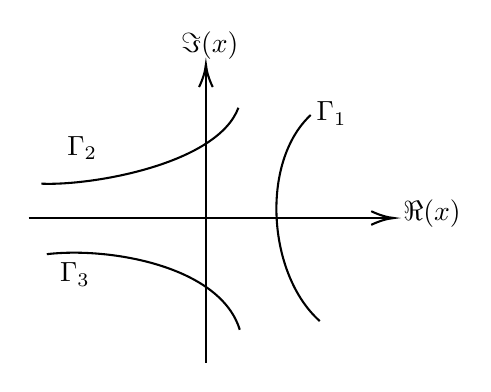
\begin{tikzpicture}[x=0.75pt,y=0.75pt,yscale=-1,xscale=1]


%Straight Lines [id:da3910937581279239] 
\draw    (530.39,290) -- (530.39,148.29) ;
\draw [shift={(530.39,146.29)}, rotate = 90] [color={rgb, 255:red, 0; green, 0; blue, 0 }  ][line width=0.75]    (10.93,-3.29) .. controls (6.95,-1.4) and (3.31,-0.3) .. (0,0) .. controls (3.31,0.3) and (6.95,1.4) .. (10.93,3.29)   ;
%Straight Lines [id:da12993081404822693] 
\draw    (445.03,220.32) -- (618.97,220.32) ;
\draw [shift={(620.97,220.32)}, rotate = 180] [color={rgb, 255:red, 0; green, 0; blue, 0 }  ][line width=0.75]    (10.93,-3.29) .. controls (6.95,-1.4) and (3.31,-0.3) .. (0,0) .. controls (3.31,0.3) and (6.95,1.4) .. (10.93,3.29)   ;
%Curve Lines [id:da4908894565729862] 
\draw    (580.9,170.68) .. controls (556.52,193.32) and (560.03,247.49) .. (585.26,269.97) ;
%Curve Lines [id:da12255840945067997] 
\draw    (546.06,167.19) .. controls (536.03,194.15) and (476.03,204.82) .. (451.13,203.77) ;
%Curve Lines [id:da8983783715640103] 
\draw    (546.7,274.15) .. controls (537.37,243.49) and (484.03,234.15) .. (453.74,237.74) ;

% Text Node
\draw (582.29,162.95) node [anchor=north west][inner sep=0.75pt]    {$\Gamma _{1}$};
% Text Node
\draw (462.1,179.5) node [anchor=north west][inner sep=0.75pt]    {$\Gamma _{2}$};
% Text Node
\draw (458.61,240.46) node [anchor=north west][inner sep=0.75pt]    {$\Gamma _{3}$};
% Text Node
\draw (624,210.11) node [anchor=north west][inner sep=0.75pt]    {$\Re ( x)$};
% Text Node
\draw (516.94,129.11) node [anchor=north west][inner sep=0.75pt]    {$\Im ( x)$};
\end{tikzpicture}
\eea
    This becomes the \emph{Airy integral}. 
    
    \item Treat the integral as an asymptotic series in $\lambda$ via
    $ \exp{\lb\frac{\lambda}{3!\hbar}x^3\rb}= \sum_{n\geq 0} \frac{\lb \frac{\lambda}{3!\hbar}x^3\rb^n}{n!}$.
\ei

\subsection{Perturbative theory}
Let's focus on method (2). This is known as the \emph{perturbative theory}. We will also add the background parameter $a$ in our integral.
\bea \int_\bR \frac{dx}{\sqrt{2\pi\hbar}}\ e^{\lb -\hf x^2+\frac{\lambda}{3!}(x+a)^3\rb /\hbar}
\ =\ e^{\frac{\hbar}{2}\partial_a^2} e^{\frac{\lambda}{3!\hbar}a^3}
\ =\ \sum_{k,m\geq 0} 
\frac{\lb \frac{\hbar}{2}\partial_a^2\rb^k}{k!}
\frac{\lb  \frac{\lambda}{3!\hbar}a^3\rb^m}{m!}.
\eea
We have used the fact (Proposition \ref{prop1}) that the integration $\int_\bR \frac{dx}{\sqrt{2\pi\hbar}} g(x+a) e^{-\frac{1}{2\hbar} x^2}$ is described by the operator $e^{\frac{\hbar}{2} \partial_a^2}g(a)$. This infinite sum can be organized into graphs (or Feynman diagrams). Here are some examples.
\begin{itemize}
    \item one term in $\lb \frac{\hbar}{2}\partial_a^2\rb^2
    \lb \frac{\lambda}{3!\hbar}a^3\rb^2$ has
    \bea
    \begin{fmffile}{fd1}
    \begin{tabular}{c}
        \begin{fmfgraph*}(120,70)
                \fmfleft{i}
                \fmfright{o}
                \fmf{plain,tension=4}{i,v1}
                \fmf{plain,tension=4}{v2,o}
                \fmf{plain,left,label=$\frac{\hbar}{2}\partial_a\otimes\partial_a$,label.side=left,tension=1}{v1,v2,v1}
                \fmfv{label=$\frac{\lambda}{\hbar}$,label.angle=120,decor.shape=circle,decor.filled=full,decor.size=2thick}{v1}
                \fmfv{label=$\frac{\lambda}{\hbar}$,label.angle=60,decor.shape=circle,decor.filled=full,decor.size=2thick}{v2}
                \fmflabel{$a$}{i}
                \fmflabel{$a$}{o}
        \end{fmfgraph*}
        \end{tabular}
    \end{fmffile}
    ~~~~~~~~ \sim\ \lambda^2 a^2,
    \eea
    
    \item one term in $\lb \frac{\hbar}{2}\partial_a^2\rb
    \lb \frac{\lambda}{3!\hbar}a^3\rb^2$ has
    \bea
    \begin{fmffile}{fd2}
    \begin{tabular}{c}
        \begin{fmfgraph*}(120,70)
                \fmfleft{i1,i2}
                \fmfright{o1,o2}
                \fmf{plain,tension=.5}{i1,v1}
                \fmf{plain,tension=.5}{i2,v1}
                \fmf{plain,tension=.5}{v2,o1}
                \fmf{plain,tension=.5}{v2,o2}
                \fmf{plain,label=$\hbar \partial_a\otimes\partial_a$,label.side=left,tension=.4}{v1,v2}
                \fmfv{label=$\frac{\lambda}{\hbar}$,label.angle=180,decor.shape=circle,decor.filled=full,decor.size=2thick}{v1}
                \fmfv{label=$\frac{\lambda}{\hbar}$,label.angle=0,decor.shape=circle,decor.filled=full,decor.size=2thick}{v2}
                \fmflabel{$a$}{i1}
                \fmflabel{$a$}{i2}
                \fmflabel{$a$}{o1}
                \fmflabel{$a$}{o2}
        \end{fmfgraph*}
        \end{tabular}
    \end{fmffile}
    ~~~~~~~~ \sim\ \frac{\lambda^2}{\hbar}a^4.
    \eea
\end{itemize}

In general, given a graph $\Gamma$, let
\bea
D &=\text{number of external edges},\\
E &=\text{number of internal edges},\\
V &=\text{number of vertices}.\\
\eea
Define a \textbf{weight function} 
\bea W_{\Gamma}(a) \coloneqq a^D\lambda^V \hbar^{E-V}.\eea
For a connected graph $\Gamma$, we have
\bea V-E= \chi(\Gamma)=1-\ell,\eea
where $\chi$ is the Euler characteristic of the graph $\Gamma$ and $\ell$ is the number of loops. Then
\bea
\boxed{W_{\Gamma}(a)=a^D \lambda^V \hbar^{\ell-1}}\ .\eea

\begin{eg}
\bea
    \begin{fmffile}{fd3}
    \begin{tabular}{c}
        \begin{fmfgraph*}(80,40)
                \fmfleft{i}
                \fmfright{o}
                \fmf{plain,tension=4}{i,v1}
                \fmf{plain,tension=4}{v2,o}
                \fmf{plain,left,tension=2}{v1,v2,v1}
                \fmfv{decor.shape=circle,decor.filled=full,decor.size=2thick}{v1}
                \fmfv{decor.shape=circle,decor.filled=full,decor.size=2thick}{v2}
        \end{fmfgraph*}
        \end{tabular}
    \end{fmffile}
    ~~~~~~~~ D=2, E=2, V=2 \RA \ell=1.
    \\ \\ 
    \begin{fmffile}{fd4}
    \begin{tabular}{c}
        \begin{fmfgraph*}(80,40)
                \fmfleft{i1,i2}
                \fmfright{o1,o2}
                \fmf{plain,tension=.5}{i1,v1}
                \fmf{plain,tension=.5}{i2,v1}
                \fmf{plain,tension=.5}{v2,o1}
                \fmf{plain,tension=.5}{v2,o2}
                \fmf{plain,tension=.4}{v1,v2}
                \fmfv{decor.shape=circle,decor.filled=full,decor.size=2thick}{v1}
                \fmfv{decor.shape=circle,decor.filled=full,decor.size=2thick}{v2}
        \end{fmfgraph*}
        \end{tabular}
    \end{fmffile}
    ~~~~~~~~ D=4, E=1, V=2 \RA \ell=0.
    \eea
\end{eg}

\begin{prop}[Feynman diagram expansion formula]
\bea \int_\bR \frac{dx}{\sqrt{2\pi\hbar}}\ e^{\lb -\hf x^2+\frac{\lambda}{3!}(x+a)^3\rb /\hbar}
\ =\ e^{\frac{\hbar}{2}\partial_a^2} e^{\frac{\lambda}{3!\hbar}a^3}
\ =\ \on{exp}\lb \sum_{\Gamma:\text{ connected trivalent graph}} \frac{W_\Gamma(a)}{\left| \on{Aut}(\Gamma)\right|}\rb.\eea
Here $\on{Aut}(\Gamma)$ is the automorphism group of $\Gamma$. 
\end{prop}

If we define
\bea W(a) &=\hbar \sum_{\Gamma:\text{ connected graph}} \frac{W_\Gamma(a)}{\left| \on{Aut}(\Gamma)\right|}\\
&=\sum_{g\geq 0}W_g(a)\hbar^g \qquad (\text{expansion in } \hbar).\eea
Here $\hbar W_\Gamma(a)\sim \hbar^{E-V+1}=\hbar^\ell.$ Then we can write the above formula as
\bea
e^{W(a)/\hbar}=\int_{\bR} \frac{dx}{\sqrt{2\pi\hbar}}\ e^{-\frac{1}{2\hbar}x^2} e^{I(x+a)/\hbar}
\eea
for $I(x)=\frac{\lambda x^3}{3!}$ is the cubic \textbf{interaction}. We can further write it as 
\bea e^{W(a)/\hbar}=e^{\frac{\hbar}{2}\partial_a^2} e^{I(a)/\hbar}\eea
and $e^{\frac{\hbar}{2}\partial_a^2}$ plays the role of \textbf{integration}. In physics terminology, we have the operator called the \textbf{propagator}:
\bea P\coloneqq \hf \partial_x^2.\eea
Define a transformation on $I(x)$:
\bea I\mapsto W(P,I)\eea
by the equation
\bea e^{W(P,I)/\hbar}\coloneqq e^{\hbar P}e^{I/\hbar}.\eea
Similarly, we have a graph formula
\bea
W(P,I)=\hbar \sum_{\Gamma:\text{ connected graph}} \frac{W_\Gamma}{\left| \on{Aut}(\Gamma)\right|}.\\
\eea
In general, $I(x)$ involves higher power interaction terms. For example, we have 
\bea
    \begin{fmffile}{fd5}
    \begin{tabular}{c}
        \begin{fmfgraph*}(80,40)
                \fmfleft{i}
                \fmfright{o}
                \fmf{plain,tension=4}{i,v1}
                \fmf{plain,tension=4}{v2,o}
                \fmf{plain,left,label.side=left,tension=2}{v1,v2,v1}
                \fmfv{decor.shape=circle,decor.filled=full,decor.size=2thick}{v1}
                \fmfv{decor.shape=circle,decor.filled=full,decor.size=2thick}{v2}
        \end{fmfgraph*}
        \end{tabular}
    \end{fmffile}
    ~~ + ~~
    \begin{fmffile}{fd6}
    \begin{tabular}{c}
        \begin{fmfgraph*}(80,40)
                \fmfleft{i1,i2}
                \fmfright{o1,o2}
                \fmf{plain,tension=4}{i1,v1}
                \fmf{plain,tension=4}{i2,v1}
                \fmf{plain,tension=4}{v2,o1}
               \fmf{plain,tension=4}{v2,o2} \fmf{plain,left,label.side=left,tension=3}{v1,v2,v1}
                \fmfv{decor.shape=circle,decor.filled=full,decor.size=2thick}{v1}
                \fmfv{decor.shape=circle,decor.filled=full,decor.size=2thick}{v2}
        \end{fmfgraph*}
        \end{tabular}
    \end{fmffile}
    ~~ +\ \cdots. ~~
\eea

\begin{prop}
$W(P,-)$ defines a transformation on
\bea W(P,-): \bR[[ x,\hbar]]^+ \to \bR[[ x,\hbar]]^+,\eea
where $\bR[[  x,\hbar]] ^+\coloneqq x^3 \bR[[ x]] \oplus \hbar \bR[[ x,\hbar]] $ are the \emph{terms at least cubic modulo $\hbar$}. $W(P,-)$ is also the renormalization group (RG) flow operator with respect to the propagator $P$.
\end{prop}

\noindent \textsc{References}:
\cite{sili2015introqft}, \cite{costello2011renormalization} for the RG flow operator,
\cite{bessis1980quantum} for diagram techniques.
